\pagenumbering{roman}
%%%%%%%%%%%%%%%%%%%%%%%%%%%
% Diplomaterv-kiiras (ezt adjak, bele kell kötni a diplomába)
%%%%%%%%%%%%%%%%%%%%%%%%%%%
\begin{center}

\textbf{BUDAPEST UNIVERSITY OF TECHNOLOGY AND ECONOMICS}

\medskip


\includegraphics[width=8.79cm]{images/bme.pdf}

\medskip

\textbf{FACULTY OF ELECTRICAL ENGINEERING AND INFORMATICS\\SOFTWARE ENGINEERING}

 \vspace{2cm}
 \Large\textbf{\cim}

 \vspace{6mm}
 \textbf{\nev} \\
 \texttt{\href{mailto:vsza@vsza.hu}{<vsza@vsza.hu>}} \\ \strut \\

 \Large\textbf{THESIS STUDY}

\end{center}

\vfill

Consultant:

\begin{center}
\konzulens\\ \konzbeoszt

\vspace{96pt}

December 2011
\end{center}

% \vspace{6mm}
% \begin{tabular}{p{80mm}l}
% A záróvizsga tárgyai:   & Első tárgy \\
%                         & Második tárgy \\
%                         & Harmadik tárgy
%  \end{tabular}
%
%  \vspace{6mm}
%  \begin{tabular}{p{80mm}l}
%  A tervfeladat kiadásának napja:         &  \\
%  A tervfeladat beadásának határideje:    &
%  \end{tabular}
%
% \vfill
%
% \begin{center}
% \begin{tabular}{cc}
%  \makebox[7cm]{\emph{dr.\ Görgényi András}}    & \makebox[7cm]{\emph{dr.\ Péceli Gábor}} \\
%  \makebox[7cm]{adjunktus, diplomaterv felelős} & \makebox[7cm]{egyetemi tanár, tanszékvezető}
% \end{tabular}
% \end{center}
%
%  \vspace{6mm}
%  \begin{tabular}{p{80mm}l}
%  A tervet bevette:           & \\
%  A terv beadásának dátuma:   & \\
%  A terv bírálója:            &
%  \end{tabular}


 \thispagestyle{empty}
 \blankpage

\selectlanguage{magyar}
%%%%%%%%%%%%%%%%%%%%%%%%%%%
% Diplomaterv-kiiras melleklete (ezt is adjak, bele kell kötni a diplomába)
%%%%%%%%%%%%%%%%%%%%%%%%%%%
 \begin{textblock*}{\paperwidth}(0mm,0mm)
    \noindent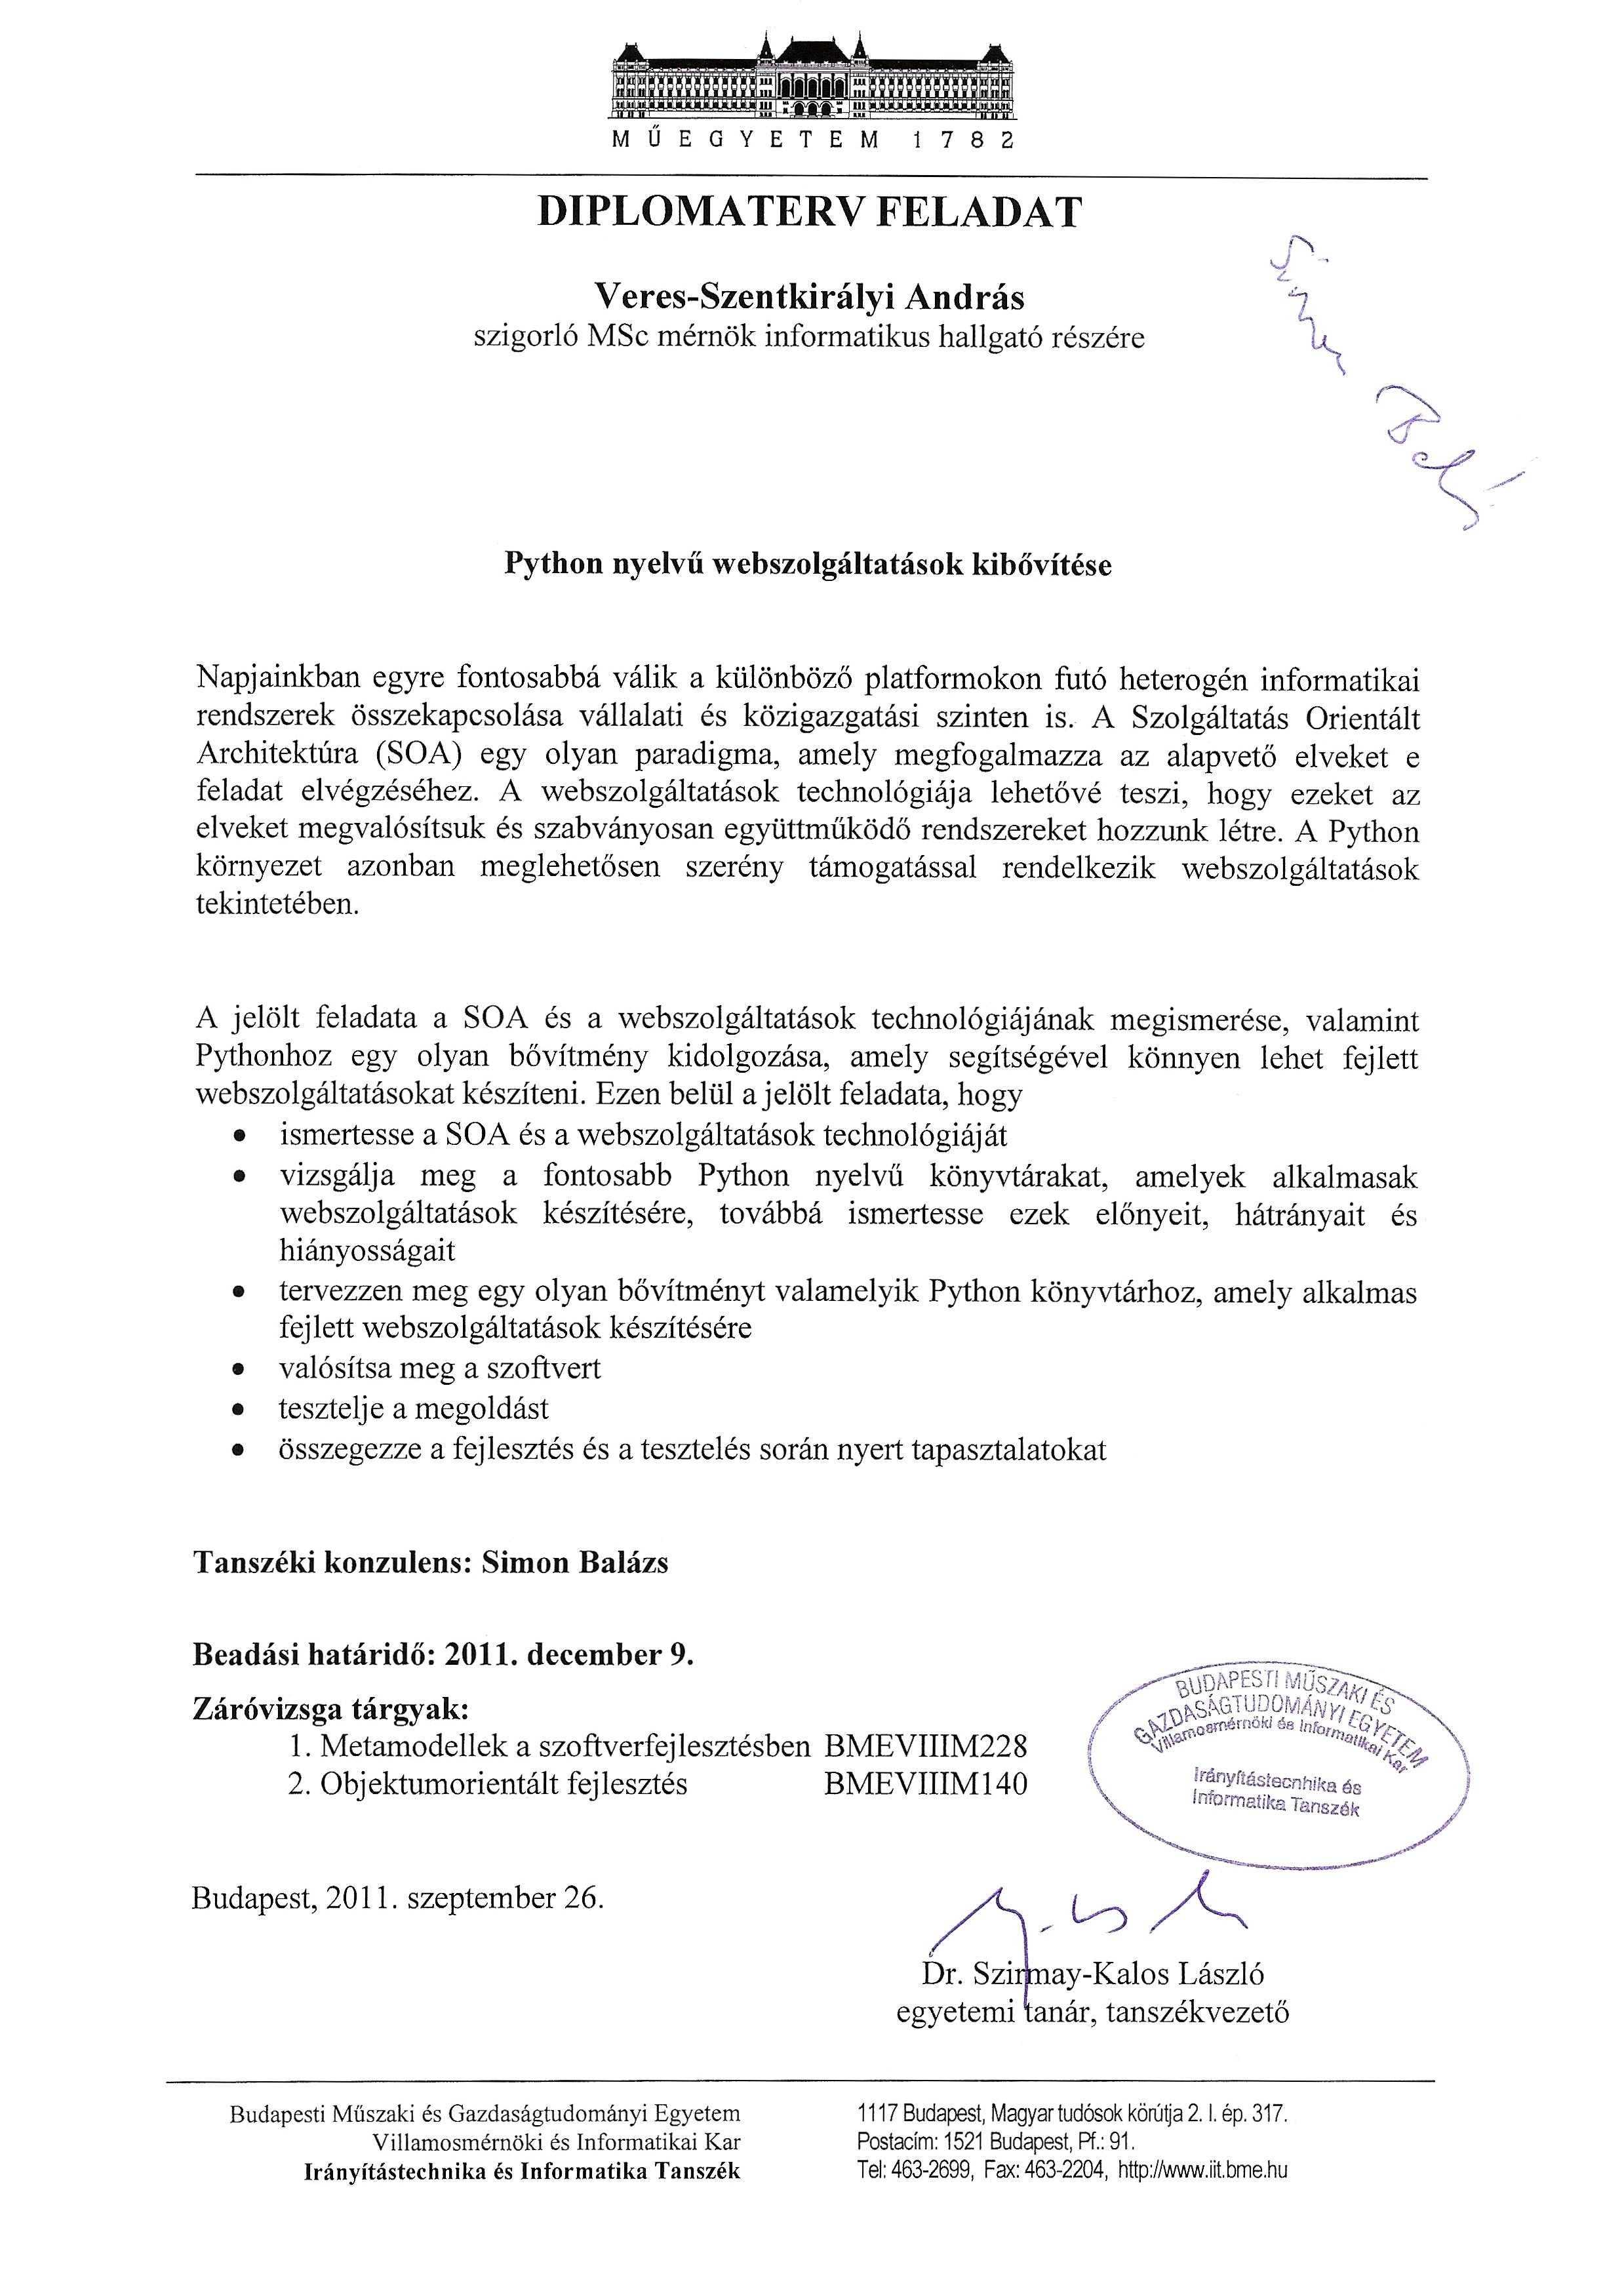
\includegraphics[width=\paperwidth,height=\paperheight]{images/feladat-retouched.jpg}
	\end{textblock*}
	\mbox{}
 \blankpage

%%%%%%%%%%%%%%%%%%%%%%%%%%%
% Nyilatkozat
%%%%%%%%%%%%%%%%%%%%%%%%%%%
\def\abstractname{Nyilatkozat}
\begin{abstract}

\noindent
Alulírott \emph{Veres-Szentkirályi András}, szigorló hallgató kijelentem,
hogy ezt a diplomatervet meg nem engedett segítség nélkül, saját  magam
készítettem, csak a megadott forrásokat (szakirodalom, eszközök, stb.)
használtam fel. Minden olyan  részt, amelyet szó szerint, vagy azonos
értelemben, de átfogalmazva más forrásból átvettem, egyértelműen, a
forrás megadásával megjelöltem.

Hozzájárulok, hogy a jelen munkám alapadatait (szerző(k), cím, angol és magyar
nyelvű tartalmi kivonat, készítés éve, konzulens(ek) neve) a BME VIK nyilvánosan
hozzáférhető elektronikus formában, a munka teljes szövegét pedig az egyetem
belső hálózatán keresztül (vagy autentikált felhasználók számára) közzétegye.
Kijelentem, hogy a benyújtott munka és annak elektronikus verziója megegyezik.
Dékáni engedéllyel titkosított diplomatervek esetén a dolgozat szövege csak 3 év
eltelte után válik hozzáférhetővé.
\begin{flushright}
 \vspace*{1cm}
 \makebox[7cm]{\rule{6cm}{.4pt}}\\
 \makebox[7cm]{\emph{Veres-Szentkirályi András}}\\
 \makebox[7cm]{hallgató}
\end{flushright}
\end{abstract}

%%%%%%%%%%%%%%%%%%%%%%%%%%%
% Tartalomjegyzek
%%%%%%%%%%%%%%%%%%%%%%%%%%%
\selectlanguage{english}
\tableofcontents

%%%%%%%%%%%%%%%%%%%%%%%%%%%
% Kivonat
%%%%%%%%%%%%%%%%%%%%%%%%%%%
\def\abstractname{Kivonat}
\selectlanguage{magyar}
\begin{abstract}
\addcontentsline{toc}{chapter}{Kivonat}
``Én távolabbra láthattam, de csak azért, mert óriások vállán álltam'' -- Isaac Newton több mint 300 éves üzenete jól illeszthető a szolgáltatások együttműködésének kialakítása mögött rejlő motivációval. Ahogy egyre fejlettebb szolgáltatások kerültek a piacra, a versenyelőny megtartásának egy jó módja ezek összekapcsolása, ezáltal újszerű, összetett termékek létrehozása. A technológia folyamatos fejlődése egyszerre teremtett sok-sok eltérő platformot és az ezek közti hatékony együttműködést lehetővé tévő szabványokat, mint a DCOM, a CORBA és az XML-RPC.

A bábeli zűrzavarra megoldás a webszolgáltatások technológiája, mely a SOAP-ot használja az üzleti üzenetek szabványos kódolására, és a világháló kapcsán már bevált, egyszerű és kiforrott szállítási mechanizmusok segítségével juttatja el azokat a címzetthez. Bár az Internet nyíltsága végtelen lehetőségeket rejt, megvannak a veszélyei is, így további szabványok jelentek meg, többek között az üzenetek hitelességének biztosítására.

Bár a nyílt szabványok, mint a SOAP, WSDL és társai egy platform-független megoldást alapozhattak volna meg, ezek fejlesztői környezetek körében élvezett támogatása közel sem egyenletes. Például a Python, egy valódi közösségi projekt, a szükséges minimumnál alig nyújt több támogatást fejlett SOAP webszolgáltatások készítéséhez, így az ezt igénylő projektek körében kevésbé népszerű választás, egyéb pozitív tulajdonságai ellenére.

Diplomatervemben bemutatom a Szolgáltatás Orientált Architektúra történetét és elveit, majd részletezésre kerülnek a webszolgáltatások, azon belül is a fejlettek. A Python környezetről is lehull a lepel, többek között áttekintem a jelenleg rendelkezésre álló, SOA megoldások készítésére alkalmas könyvtárakat mind szolgáltatási, mind fogyasztói oldalról. A felsorolást egy összegzés zárja, mellyel célom rávilágítani a fejlesztések szükségességére.

Az általam továbbfejlesztésre kiválasztott könyvtár, a SUDS bemutatása során mind a magas szintű fejlesztői interfész, mind a belső működés áttekintésre kerül, rámutatva a bővítés kiindulópontjaként használható csonka részekre. A bővítményre vonatkozó terveim és azok megvalósításának bemutatását követően szó esik a tesztkörnyezetről is, melynek elkészítésével az volt a célom, hogy bebizonyosodjon, a fejlesztés eredménye teljesíti a legfontosabb követelményt: az interoperabilitást. Végül a megoldás színvonala a felhasznált idő és hálózati forgalom mértéke alapján került értékelésre, a diplomatervet pedig tapasztalataim összegzése és továbbfejlesztési lehetőségek zárják.
\end{abstract}


%%%%%%%%%%%%%%%%%%%%%%%%%%%
% Abstract
%%%%%%%%%%%%%%%%%%%%%%%%%%%
\selectlanguage{english}
\begin{abstract}
\addcontentsline{toc}{chapter}{Abstract}
``If I have seen further it is only by standing on the shoulders of giants'' -- Isaac Newton's more than 300-year-old message is a great parallel with the motivation behind service interoperation. As more advanced services were developed, one way of improving them was to interconnect them to combine their powers into more exciting products. Continuous advancement of technology created diverging platforms, and simultaneously provided standards allowing efficient co-operation such as DCOM, CORBA and XML-RPC.

One of the solutions for this Babel-like chaos were web services using SOAP to encode business messages in a standardized way and to reuse simple and mature transport mechanisms proven useful by the World Wide Web to carry them between the recipients. While the openness of Internet offers vast opportunities, it also has its dangers, which caused additional standards to be developed, among others, for message authenticity.

Although the open standards of SOAP, WSDL and others could have been the foundation of a platform-independent solution, not every environment used for software development supports it equally. Python, a truly community-driven project is one of them, providing little more than minimal support for advanced SOAP web services, making it a less favored selection for projects needing this capability, despite its unique treats.

In this thesis, the history and principles of Service-Oriented Architecture are presented, then the scope is focused on web services, and further on to advanced ones. Then the Python environment is introduced, including the current libraries for implementing SOA solutions both on the service and consumer side. This part ends with a quick summary that makes the reasons for improvements clear.

My selection for improvement, SUDS is presented next, looking at both its high-level view and its internals, showing the possible stubs awaiting improvement. The plans and implementation details of my enhancements are introduced right after, including a testbed to make sure the new features fulfill the most important requirement: interoperation. In the end, the whole solution is evaluated using measurements of both timing and network traffic, concluding the thesis with my observations and ideas for future improvement.
\end{abstract}

\selectlanguage{magyar}
\chapter*{Magyar nyelvű összefoglalás}
\addcontentsline{toc}{chapter}{Magyar nyelvű összefoglalás}

A SOA megjelenése mögötti fő motivációt a XX. század végére kialakult informatikai világ interoperabilitási, újrafelhasználhatósági és egyéb problémáinak felszámolása jelentette. Rendszerszintű probléma lévén, a megoldást is ilyen szinten kell keresni -- egy ideális szolgáltatás-orientált megoldás elemei lazán csatoltak, és a köztük történő kommunikáció jól definiált, szabványos módon zajlik. Visszatekintve a szoftvertechnológia történelmére, ez a paradigmaváltás szépen illeszkedik a függvények, objektumok, komponensek alkotta lánc végére, ezáltal megoldást nyújtva az egyre összetettebb rendszerek kezelhetőségének problémájára.

Mint neve is mutatja, a SOA inkább elveket fogalmaz meg, technológia-specifikus elemeket szándékosan nem említ, így több szervezet is próbálkozott a megvalósítással. A Microsoft DCOM-ja és az OMG CORBA-ja is többé-kevésbé szabványos módon próbált együttműködési lehetőséget biztosítani entitások között -- utóbbiak valahol a komponens és a szolgáltatás közti skálán mozogtak, definíciótól függően. E korai megoldások alkalmazásának azonban megvoltak a maguk korlátai; a DCOM értelemszerűen Windows platformot igényel, a CORBA-t implementáló ORB-ok pedig ugyan sokszínűek OS támogatás és licensz szempontjából, azonban az egyes megoldások közti együttműködés nem mindig problémamentes.

További fejtörést okoz, hogy bizonyos szintű együttműködés felett a kommunikációnak -- szemben a belső vállalati hálózattal -- a nyílt Interneten kell zajlania, ahol a közvetlen TCP kapcsolatokon keresztüli bináris adatcsere az üzemeltetők ``rémálma''. Időközben megjelent a világháló, magával hozva a HTTP-t mint kifejezetten Interneten keresztüli működésre tervezett adattovábbító protokollt, melynek forgalma a hálózathatáron proxy szerverekkel szűrhető és átalakítható. Ezen és más jó tulajdonságai (pl.\ tartalomtól független adattovábbítás) miatt az együttműködés egyik alapkövévé vált.

A definíciókat szabadon értelmezve minden ilyen, HTTP felett elérhető szolgáltatást webszolgáltatásnak tekinthetünk. Az első ilyen az XML-RPC volt, nevéből eredő módon távoli eljáráshívás szemantikáját követve. Működése igen egyszerű volt, ennek köszönhetően igen széles támogatottságra tett szert. A Microsoft berkein belül azonban nem elégedtek meg ennyivel, és további fejlesztés során létrehozták a SOAP-ot, mely első ránézésre nem sokban különbözik elődjétől.

\bigskip

A kiadott szabvány kezelését átvette a W3C, a SOAP pedig a webszolgáltatások egyik elterjedt kódolásává vált, szállítási célra HTTP(S) vagy SMTP protokollt használva. Szintén XML alapon kialakult a WSDL, mely képes a szolgáltatás interfészét egy gépi módon feldolgozható formában leírni. Szolgáltatások esetében általában forráskód alapján automatizáltan generálható, kliensek esetén pedig a fejlesztő számára az adott környezethez illeszkedő wrapperek hozhatók létre, akár dinamikusan, akár előzetes kódgenerálással.

A fejlődés persze nem állt meg, a W3C és az OASIS további -- metaadat cserét adót, biztonságot, megbízhatóságot javító -- szabványokkal egészítette ki a családot, az ily módon emelt színvonalú szolgáltatásokat nevezzük fejlettnek. Ezek előnye, hogy szabványos módon lehetséges magas minőségű szolgáltatások létrehozása, miközben a kód továbbra is az üzleti logikára fókuszál. Érdemes azonban megjegyezni, hogy az összetett, folyamatosan fejlődő szabványokat nem minden implementáció követi azonos mértékben, így sérülhet az interoperabilitás és a platformfüggetlenség.

A biztonság az egyik terület, amely többé-kevésbé elterjedt fejlett webszolgáltatás szabványokkal lefedésre került. Bár HTTP feletti protokoll biztonsága esetében logikusnak tűnhet a HTTPS használata, sokszor előfordul olyan hálózati környezet, ahol proxy-kon is áthalad a forgalom, így ez a megoldás nem alkalmas végponttól végpontig terjedő biztonságos (azonosított felek között zajló, digitálisan aláírt és/vagy titkosított) csatorna létrehozására. Az IBM, a Microsoft és a Verisign 2002-ben kifejlesztett egy szabványt, melynek végső formáját 2004-ben adta ki az OASIS, WS\hyp{}Security néven. E megoldás képes a kérést indító felhasználó azonosítására, valamint üzenet egy részhalmazának elektronikus aláírására és/vagy titkosítására is.

\bigskip

A Python besorolását tekintve interpretált, objektum-orientált programozási nyelv, jellegzetes tulajdonságai azonban egyértelműen megkülönböztetik hasonló ``társaitól''. Szokatlannak hathat például az indentálás használata a forráskód strukturálásának céljára, holott jobban belegondolva hosszú távon olvashatóbbá teszi a mások által írt kódot, növelve az esélyét az újrafelhasználásnak. A nyelv tervezési és továbbfejlesztési elveit jól összefoglalja egy egyszerű kifejezés, melyből előnyei és hátrányai is levezethetők: ``futtatható pszeudokód'' -- azaz egy átlagos Python kódrészlet kellően explicit ahhoz, hogy bárki (akár Python tudás nélkül is) átlássa működését.

Futtatókörnyezetként gyakran a CPython nevű referencia implementációt használják, mely a legtöbb operációs rendszerre elérhető, több UNIX-szerű disztribúció alapértelmezésként szállítja, mivel tervezésénél fogva szkriptelési célra is használható UNIX shebang használatával. Emellett azonban léteznek projektek Python forráskódból Java és .NET bájtkód előállítására, valamint a Nokia támogatásával elkészült egy port a Nokia S60 (Symbian) platformra is.

A letölthető Python disztribúciók egy meglehetősen teljes könyvtárkészlettel érkeznek, beépített megoldást tartalmazva a legtöbb, fejlesztő által igényelt célra, mint fájlok, hálózati kapcsolatok és különböző formátumok kezelése. Ezek implementációja készülhet tisztán Python nyelven -- mely esetben az összes fent említett platformon működőképes a megoldás módosítás nélkül -- vagy a C/C++ API használatával. Utóbbi megoldás használatával natív API-k is elérhetővé tehetők Python objektumok szintjén, az ilyen könyvtárakat bindingnek nevezzük, ezek segítségével oldható meg, hogy az egyébként interpretált nyelvekre jellemző teljesítménybeli kihívások hatása minimális legyen azáltal, hogy interpretált szinten csak a magas szintű logika kerül implementálásra. E tulajdonság a fejlesztőket is megfelelő irányba tereli, így elkerülhető az idő előtti optimalizációs kísérletek gyakori hibája, és lehetővé válik a gyorsan elkészült prototípus későbbi teljesítményhangolása az alapok ``kidobása'' nélkül.

\bigskip

A Pythont körülvevő igazi szabad szoftveres közösség leginkább olyan könyvtárakat készít kedvenc környezetéhez, mely vagy különösen érdekli, vagy éppen szüksége van rá, ennek következményei kedvezők az alapkönyvtárak szempontjából -- kevésbé jók azonban a SOAP-ra nézve. A távoli eljáráshívás legtöbb módjára létezik már Python megoldás, azonban a SOAP támogatása megrekedt egy bizonyos szinten -- az egyszerű alappéldák működnek, azonban a megvalósítások határaiból megsejthető az azt készítő fejlesztő igényszintje.

E helyzetért részben a hálózati hatás okolható: ha mindenki .NET-et vagy Java-t használ webszolgáltatásokon keresztüli együttműködésre, sokak számára triviális választás a két ``mammut'' egyike. Szintén része a problémának a Pythonnal fejlesztők gondolkodásmódja, mely kisebb, autonóm egységekből való építkezésben gondolkozik, melyek között a kommunikáció egyszerű protokollokkal zajlik -- és valljuk be, ezen peremfeltételekről nem a SOAP az első, ami eszünkbe jut. Természetesen léteznek Python SOA fejlesztők és munkájuk eredményeként több megoldás is elérhető.

A két ``nagy öreg'' a \emph{SOAPy} és a \emph{ZSI}, ám ezek mára jelentősen vesztettek fényükből, előbbi inkompatíbilis is frissebb Python kiadásokkal, utóbbi pedig bár működik, használata nehézkes, fejlesztése gyakorlatilag karbantartásra korlátozódik. Újabb megoldás a \emph{soaplib} -- \emph{rpclib} páros, mely inkább szolgáltatások készítésére alkalmas, arra viszont nagyon kényelmesen használható. Jó párja a \emph{SUDS}, mely inkább kliensoldali funkcionalitásban jeleskedik, használata kényelmes és intuitív, jól segíti a fejlesztőt mind prototípus elkészítésében, mind kész rendszerben használva. Kakukktojás a \emph{sec-wall}, mely szolgáltatások ``fejlesztését'' teszi lehetővé olyan szempontból, hogy proxyként egy szolgáltatás és a kliensek közé állítva fejlett tulajdonságokkal ruházza fel előbbit, a biztonságot és a teljesítményt szem előtt tartva.

\bigskip

Szakmai gyakorlat során a \emph{sec-wall} szoftver fejlesztésében vettem részt, így diplomatervemben a kliensoldalra koncentrálva a SUDS-ot kezdtem el tanulmányozni, mely jelenleg a Python környezet de facto SOAP kliens megoldásának tekinthető. Működési módja jó kompromisszum a kényelmes és gyors prototípus építés és a hatékonyv működés között -- egy WSDL címének birtokában proxy objektumot hoz létre, majd az ezen végzett metódushívások hatására a Python dinamikus metódusfeloldási lehetőségeit kihasználva generálja a SOAP kéréseket. Az összetett típusok példányosítása és a kódgenerálás hiánya közti ellentmondást a \emph{Factory} tervezési mintával oldja fel, a kliens objektumtól név szerint kérhető a WSDL-ben (vagy az általa hivatkozott sémákban) definiált osztályok létrehozása.

A dokumentáció és a forráskód tanulmányozásával felfedeztem a SUDS belső felépítését, kezdve a kliens proxy létrehozásától a metódushívásokon keresztül a csatornamodellig. Kiderült többek között, hogy történelmi okokból például saját DOM implementációt használ a könyvtár, melynek cseréje kompatíbilitási okokból jelenleg lenne kifizetődő. Kipróbáltam a WS\hyp{}Security támogatást is, mely létezik ugyan, ám igencsak korlátozott. Az azonosításra használható UsernameToken támogatás hiányos volt és a szabványt sem tartotta be teljesen, digitális aláírásra pedig egyáltalán nem volt mód. Szerencsére az utóbbi verziókban került egy plugin megoldás is a SUDS-ba, melynek használatával külső komponensekkel bővíthető a megoldás tudása anélkül, hogy a kódot módosítani kellene. Az ily módon betöltött és regisztrált külső komponensek értesítést kaphatnak és befolyásolhatják a működést a kliens életciklusának összes fontosabb pontján, így ideális megoldás a funkcionalitás bővítésére.

\bigskip

A fejlesztés első lépéseként szabványkövetővé tettem a UsernameToken implementációt, megoldva a \emph{digest} módú jelszóküldést is, melyet a korábbi verzióban a felhasználónak kézzel kellett megadnia. Ehhez természetesen a könyvtár kódját kellett módosítani, így azonban legalább kiismertem magam a WS\hyp{}Security modulban.

A második, nagyobb lépés a digitális aláírás lehetőségének megteremtése volt. Ennek megvalósítására olyan plugint készítettem, mely közvetlenül az üzenet elküldése előtt kapja meg a vezérlést, így bemenetként is nyers bájtfolyamot kap, kimenete pedig közvetlenül a hálózatra kerül. E tervezési döntés előnye, hogy nem kell a SUDS saját DOM implementációjának korlátait figyelni, valamint a használható könyvtárak halmazát is bővíti. Mivel nem akartam a kereket újra feltalálni, nekiálltam keresni már létező könyvtárakat, melyek legalább a funkcionalitás egy részét készen tartalmazzák, kiemelt figyelemmel kezelve a natív kódú megoldásokat.

Az XML feldolgozásának céljára a natív kódú \emph{libxml2} könyvtárat, Python részről pedig a \emph{python-libxml2} -- \emph{LXML} párost választottam. A natív alapkönyvtár gyors, elterjedtsége miatt megbízhatónak tekinthető, és az OASIS XML tesztjeit kivétel nélkül teljesíti. Előbbi Python binding teljes funkcionalitásá elérhetővé teszi, cserébe az API nagyban C jelleget hordoz magában, utóbbi egy részhalmazt ad csak a fejlesztő kezébe, cserébe azt magasabb szintű OO rétegbe csomagolja -- jó példa a különbségre a hibák egyik esetben visszatérési értékkel, másik esetben kivétellel való jelzése.

Kriptográfiai feladatok megoldására az \emph{OpenSSL} könyvtárat és \emph{pyOpenSSL} bindingjét választottam, mivel jól karbantartott, szintén elterjedt implementációk, előbbi a FIPS 140-2-nek is megfelel. Közvetlenül jelenleg kizárólag arra a célra használom, hogy PEM fájlokat tudjon beolvasni, mégis tapasztalataim alapján ez az egyetlen könyvtár, ami ezt megfelelően támogatja.

A feladat lényegét, az XML digitális aláírást az \emph{XMLSec} könyvtárra és \emph{PyXMLSec} bindingjére bíztam. Előbbi mai napig jól karbantartott szoftver, libxml2-t és OpenSSL-t használ részfeladatokra, bár utóbbi helyett alternatív könyvtárakat is támogat. Sajnos azonban a Python bindingek még 2003-ban készültek egy francia projekt kapcsán, 2005 óta nem fejlesztik, ennek ellenére azonban működésre bírható, a teljes -- általam igényelt -- funkcionalitáshoz egy, a projekt levelezőlistájára 2010-ben érkezett patch-re volt szükség. A dokumentáció hiányosságai miatt használata kísérletezést igényel, azonban tapasztalataim alapján egyelőre ez az egyetlen Python megoldás, amely valóban képes XML aláírások készítésére -- létezik több, kiváltására törekvő projekt, de mind többé-kevésbé messze áll még a teljességtől.

Mint fentebb említettem, a megvalósított Python komponens bementként a már bájtsorozattá szerializált SOAP kéréshez fér hozzá, ebbe először LXML segítségével beszúrja a WS\hyp{}Security által előírt digitális aláírási struktúrát, üresen hagyott értékekkel. Ezt követően az XML ismét szerializálásra kerül, majd az eredményen az XMLSec könyvtár elvégzi a konkrét aláírást, a SOAP ismerete nélkül, kizárólag a számára előkészített ``biankó'' struktúrát használva. Az XMLSec libxml2 fán képes dolgozni, így ezzel történik a beolvasás, majd az aláírást követően a szerializáció is, melynek kimenetével lecserélésre kerül az eredeti kérés, így a hálózaton már egy aláírt kérés kerül továbbításra. A natív erőforrások hatékony használata érdekében ``becsomagoltam'' a libxml2 által épített fát és az XMLSec aláírási kontextus objektumát is, mivel a Python szemétgyűjtése ilyenkor nem kielégítő.

\bigskip

Egy elkészült SOA megoldás természetesen csak akkor ér valamit, ha képes együttműködni más megvalósításokkal is. Ennek tesztelésére egy saját környezetet építettem \emph{Arena} néven, mely referencia implementációként egy \emph{Apache CXF} webszolgáltatást képes létrehozni dinamikusan, majd választhatóan szintén CXF vagy SUDS klienssel hívja meg annak tesztelési célú metódusát. A konfiguráció egyszerű szöveges, JSON formátumú fájlokkal végezhető, a kulcsokat pedig egy \emph{make} alapú rendszerrel lehet generálni a különböző komponensek által elvárt formátumban, így elkerülhetők a lejáró statikus tanúsítványok okozta problémák.

Az aláíró komponens első működőképes változatának elkészülte után ezt a tesztkörnyezetet használtam a mérések elvégzésére is, ennek megfelelően támogatást adtam hozzá különböző konfigurációk kezelésére mind biztonság, mind kérések számának szempontjából. A környezet mérte az egyes kódrészek futásához szükséges időt, a hálózati forgalmat pedig a \emph{Wireshark} eszközzel rögzítettem és analizáltam később. Azonos funkcionalitású Python alternatíva híján méréseim során a SUDS minőségi mutatóit az Apache CXF-éivel hasonlítottam össze.

A hálózati forgalom mérése során arra jutottam, hogy a SUDS egy olyan HTTP könyvtárat használ, mely nem támogatja a protokoll \emph{keep-alive} opcióját, mely lehetővé tenné, hogy ne épüljön ki minden egyes kéréshez egy újabb TCP kapcsolat. Bár ez elsőre nem tűnhet nagy különbségnek, 100 kérés esetén már két és félszer annyi csomagot cserélt a SUDS a szolgáltatással, mint a CXF esetében, mely támogatja ezt a lehetőséget.

Az proxy példányosítás idejénél azt mértem, mennyi idő telik el a kliens indulásától addig, hogy rendelkezésre áll egy proxy objektumra mutató referencia. Minden konfiguráció esetében kevesebb mint félidő alatt végez a SUDS a CXF-fel szemben, emellett érdekes, hogy digitális aláírás esetében átlagosan további 210 ms-ba kerül a komponens inicializálása, miközben a CXF inicializálása ilyenkor is nagyságrendileg ugyanannyi időt igényel. Egy logikus magyarázat a jelenségre a könyvtárak kizárólag igény esetén történő megoldása.

A másik mért idő a proxy rendelkezésére állását követően egy-egy kérés teljes lefutásához szükséges időtartam. Ehhez 1, 10 és 100 kérést futtattam minden egyes konfiguráció esetében, hogy a fix és változó költségek jól látszódjanak. Az eredményekből látszik, hogy egy-egy kérés indítása esetén még kétszer annyi időbe telik a CXF számára a hívás, a kérések számának növelésével azonban ``olvad'' az előny, 100 kérés esetén már a CXF teljesít jobban, igaz, csak 1-5\%-kal. Digitális aláírás esetén azonban még 100 üzenetnél is 10\%-kal kevesebb idő alatt végez a SUDS, vélhetően a natív komponensek alkalmazásának köszönhetően.

Bár a natív komponensek használata jótékonyan hat a teljesítményre, fontos megjegyezni, hogy ezek választásakor valós rizikó, hogy alacsony szintű hibák (pl. null pointer feloldás) esetén nincs ott a menedzselt környezet ``védőhálója'', akár az egész alkalmazás futása véget érhet az operációs rendszer beavatkozása által.

\bigskip

A fejlesztés és tesztelés végeztével úgy értékelem, sikerült egy megfelelő teljesítményű terméket alkotni, azonban van még bőven lehetőség ennek fejlesztésére. Rövidtávon a HTTP keep-alive opció kihasználása javíthat a teljesítményen, középtávon pedig megvalósításra kerülhet az XML titkosítás is, melynek implementálását a jelenlegi szabvány biztonsági problémái miatt hagytam ki. Végül hosszú távon bővíthető lenne a digitális aláírásra használható algoritmusok köre -- bár a jelenleg támogatott RSA és DSA valóban lefedi a gyakori felhasználási módokat, az XML aláírásról szóló szabvány támogatja pl.\ az OpenPGP használatát is.

\selectlanguage{english}
